\chapter{Experiment}
% The details of CEBAF, CLAS, and E1-F.
Jefferson National Lab houses the continuous electron beam accelerator facility (CEBAF) which is currently capable of providing 11 GeV electron beams to three experimental end stations, and 12 GeV to a fourth.  The data analyzed in this study are from the run period E1-F, which occurred (along with several other runs) before the 12 GeV CEBAF upgrade.  The details in this chapter describe the accelerator and CLAS detector at the time of the E1-F run period.  \\

\section{CEBAF} 
Proposed in 1982 and constructed between 1987-1997 the CEBAF accelerator at Jefferson lab was composed of a pair of linear accelerators and 9 recirculating arcs arranged in a racetrack shape \cite{hardware-leemann:2001, hardware-chao:2011}.  Originally designed to provide 4 GeV unpolarized electrons to three experimental halls, CEBAF was fitted with twin polarized electron guns, and upgraded to 6 GeV beam energy before the E1-F run period.  CEBAF was built to provide an extremely high duty factor and an average beam current of up to $200 \; \mu A$.\\

\easyFigure{image/diagrams/cebaf.jpg}{Diagrammatic representation of CEBAF.}

\subsection{Electron Injection \& Polarization}
CEBAF's injector provided 45 MeV electrons with 70\%-80\% longitudinal polarization for the main accelerator.  In order to provide an apparent continuous stream of events to the detectors, electron bunches were produced at a rate of $f = 1497 \; Mhz$.  To accommodate different requests for energy and beam current simultaneously, the injector produced three interspersed bunch trains at a frequency of $499 \; Mhz$.  The output injector energy $E = 45 \; MeV$ was chosen so that injected electrons were \textit{sufficiently relativistic}.  In other words, when bunches of electrons at different energies simultaneously passed through the linear accelerators (LINACs), the relative phase difference (between different energy passes) accumulated over the distance remained less than $1^\circ$. \\

During early accelerator construction, the need for polarized electrons became apparent and the final polarized electron gun was produced in 2000.  Production of polarized electrons was achieved by using twin polarized electron guns mounted at $15^\circ$ with respect to the injector beam axis.  Inside of each gun, electrons were liberated from gallium arsenide photo-cathodes by three independent diode lasers operated at a repetition rate of $499 \; Mhz$.  During polarized production, the diodes operated at a central wavelength of $850 \; nm$.  By manipulating the laser polarization using a Pockels cell, the electron  beam spin is flipped at a rate of $60 \; Hz$.  Throughout the run period, an overall phase difference could be introduced by rotation of a wave-plate.  As will be discussed in some detail later, changes in beam helicity due to wave-plate settings must be removed from the recorded data.  After acceleration to $5 \; MeV$ the beam polarization was measured in the injector facility using a Mott polarimeter. \\

\easyFigure{image/photos/jlab.jpg}{This aerial photograph contains annotations that show the accelerator path and the three experimental halls.}

\subsection{Acceleration of Electrons}    
The north and south LINACs were responsible for increasing the energy of the electrons from $45 \; MeV$ up to an impressive $\approx 5.7 \; GeV$ before delivery to the experimental halls A, B, and C.  In order to achieve this each bunch of electrons was accelerated through ten stages (five passes through each LINAC).  The strong electric field needed to accelerate electron bunches was confined inside of superconducting 5-cell elliptical cavities.  These cavities were machined from niobium, and operated at a temperature of $2.2^\circ \; K$.  Developed at Cornell University, the cavities were operated at $1,500 \; Mhz$ with a gradient greater than $5 \; MV/m$ and a quality factor $Q_0 \geq 3 \cdot 10^9$ (the Q factor describes the monochromaticity of the cavity and is defined $Q_0 = f_0/\Delta f$).  Each cavity was sealed inside of a cryo-unit, four such units were connected together to form an $8.5$ meter cryo-module.  Each LINAC was composed of 20 such cryo-modules connected together to increase electron energies by more than $500 \; MeV$ per pass.\\

The radio frequency (RF) that powers each cavity was sourced by a water-cooled 5 kilowatt Klystron located in groups of eight above each cryo-module.  Phase locking of each cavity with a master oscillator ensured that the difference in phase between all cavities was less than one degree. The important super conductivity was maintained by circulation of liquid helium at $2.2^\circ K$.  Production of liquid helium occurred on-site at the 5 kW helium liquefaction plant.  \\

After re-circulation of fives passes through each LINAC, full energy beams were delivered to the halls.  Bunches were separated using an RF separator before entering their respective experimental halls.  The beamline leading to the halls was also equipped with the ability to separate bunches before they completed five full passes delivering either three full energy beams, two full energy beams and one lower, or one full energy beam and two of lower energy.  This capability, combined with the flexible beam polarization and beam current provided by the injector ensured that each hall could experiment at its desired settings simultaneously.  

\section{CLAS in Jefferson Lab Experimental Hall B}
The CEBAF large acceptance spectrometer (CLAS), housed in Jefferson lab's Hall B, was used to record the E1-F dataset (as well as numerous others) that is used in this study.  Capable of detecting particles over a very large angular range, the CLAS detector covered almost the full $4\pi$ solid angle around the target region.  The detector was also designed to perform efficiently for particles with a large range of momenta between 0.5-6.0 GeV.  The overall detector design consisted of a large superconducting magnet that produced a toroidal field (this magnet was referred to as the torus), and six ideally identical \textit{sectors}.  Each sector of CLAS contained an identical set of sub-systems.  After combining information from all sub-systems and running the reconstruction algorithm, complete events are measured.  This capability made CLAS unique in comparison with the arm style spectrometers of halls A and C.  The major components of CLAS are listed below.

\easyFigure{image/diagrams/clas.png}{In this diagrammatic representation of CLAS, several important detector sub-systems are labeled.}

\subsection{CLAS Torus and Drift Chambers}
Measuring the momentum of charged particles with $p > 200 \; MeV/c$ was accomplished by measuring the curvature of the particle trajectory as it passed through the CLAS toroidal magnetic field.  Six superconducting coils were arranged $60^\circ$ apart azimuthally around the beamline to create a 2 Tesla.  The field produced, which varied from two tesla at lower angles to half a tesla at angles greater than $90^\circ$, curved charged particle trajectories in the $\theta$ direction without altering the azimuthal $\phi$ direction.  The geometry of the torus magnet guided the development of the entire spectrometer.  \\

\begin{figure}
	\centering
		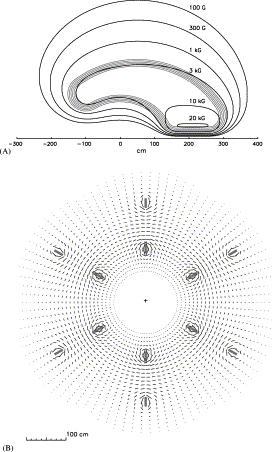
\includegraphics[width=8cm]{image/diagrams/torus-field.png}
		\caption{Diagrams of the CLAS torus field.  This figure reproduced from \cite{hardware-adams:2001}}
\end{figure}

Spatially, the 18 drift chambers were divided with 3 in each sector.  In order to perform tracking before, inside, and after the torus three radially distinct drift chambers were constructed for each sector (these were called regions 1, 2, and 3).  Each drift chamber consisted of 12 superlayers of hexagonal drift chamber cells.  Angular measurements in the azimuthal direction were accomplished by offsetting the first six and last six superlayers by $6^\circ$.  In total 35,148 individual drift chambers cells were used for tracking \cite{hardware-mestayer:2000}.

\begin{figure}
	\centering
		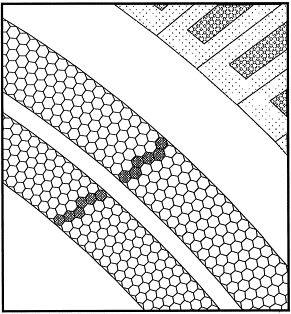
\includegraphics[width=8cm]{image/diagrams/dc-hexagonal-cells.png}
		\caption{Illustration of a charged particle interacting with cells in the drift chamber.  This figure was reproduced from \cite{hardware-mestayer:2000}}
\end{figure}
    
\subsection{CLAS Cherenkov Counter}
The Cherenkov counters (CC), located radially outside of the region 3 drift chambers, greatly assisted in the separation of electrons and negatively charged pions for tracks with momentum less than the pion momentum threshold $p < p_{\pi} \approx 2.5 \; GeV/c$ \cite{hardware-adams:2001}.  The CLAS CCs were divided into 6 sectors, like most other detectors.  Each sector was divided into 18 segments in the polar angle $\theta$ away from the beamline.  Furthermore, these segments were divided in half azimuthally to produce 12 half-sectors.  Three mirrors, a light collecting Winston cone, a magnetic shield, and a 5 inch quartz face PMT were fitted to each of the 18 segments in all 12 half-sectors.  During operation each CC was filled with $6 \; m^3$ of $C_{4} F_{10}$ gas.  The number of photo-electrons produced was recorded for tracks with polar angles between $8^\circ < \theta < 45^\circ$.  
\easyFigure{image/diagrams/cc-color.jpg}{The CLAS Cherenkov Counter.}

\subsection{CLAS Time of Flight Scintillator}
Measurements of average velocity can be made by simply knowing the distance some object has traveled in a given time period.  Operating on this principle the CLAS time of flight (TOF) system allowed for the separation of $\pi$ and $K$ for momentum $p \leq 2 \; GeV/c$.  Constructed of 57 scintillating bars per sector, the TOF system covered an impressive area of $206 \; m^2$ and spanned the range of polar angles $8^\circ \leq \theta \leq 142^\circ$.  Each of the scintillating bars measured 5.08 centimeters in thickness, 15 or 22 centimeters in width, and measured between 32 and 450 centimeters in length.  Shorter bars, which covered the relatively higher rate low scattering angle, were built with an intrinsic timing resolution of 80 picoseconds.  The timing resolution for longer bars was designed to be 160 picoseconds, and measurements performed after the detector contruction showed that the average timing resolution over the detector was 163 picoseconds \cite{hardware-smith:1999}.\\
During experiments where the electron beam was used, the start time for each event could be determined by assigning $\beta = 1$ to the fastest electron measured in the final state.  However, once the tagger magnet was powered on and photon beam was delivered on target, start time information came from the start counter.  Originally designed as six separate counters, the start counter was constructed with three counters spanning the full angular range of the detector.  The target was surrounded by these three thin scintillators which had sufficient resolution to determine the difference between two sequentially arriving bunches ($\sigma \approx 350 \; ps$). 

\subsection{CLAS Electromagnetic Calorimeter}
The outermost later of the CLAS detector was the electromagnetic calorimeter (EC).  This sampling calorimeter was a main component of the CLAS trigger and had several important roles.  Foremostly, the EC detected and triggered on electrons with $E > 0.5 \; GeV$.  Detecting neutral particles such as photons and neutrons was a secondary role.  By detecting photons with energies higher than 200 MeV, and having sufficient granular resolution, strongly decaying $(\pi^0$ or $\eta) \rightarrow \gamma \gamma$ particles were measured.  Separation of neutrons and photons was achieved by combining information from the EC with timing information from the CLAS time of flight system \cite{hardware-amarian:2001}.  \\
Structurally, the EC was composed in total of 1296 PMTs and 8424 scintillating strips in the six EC modules (one per sector).  Alternating layers of lead and scintillator material were used to create a sampling fraction $E_{dep}/p$ of approximately 0.3 for electrons.  Measuring just 10 mm thick, and with a width of 10 cm (to balance cost of PMTs and granularity), the length of the scintillating strips depended on the angular location.  Each EC module contained 3 sets of 13 layers offset by $120^\circ$ to provide spatial information, these layers were referred to as U, V, and W.  
\easyFigure{image/diagrams/ec.png}{The U, V, W structure of CLAS electromagnetic calorimeter is shown above.}

\begin{figure}
	\centering
		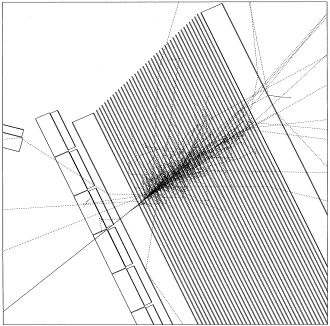
\includegraphics[width=8cm]{image/diagrams/ec-shower-geant.png}
		\caption{GEANT simulation of an electron showering in the EC.  This figure originally appeared in \cite{hardware-amarian:2001}}
\end{figure}
